\documentclass[12pt, a4paper]{article}
\usepackage[utf8]{inputenc}
\usepackage{geometry}
\geometry{top=2.5cm, bottom=2.5cm, left=2.5cm, right=2.5cm}
\usepackage{graphicx}
\usepackage{tabularx}
\usepackage{booktabs}
\usepackage{hyperref}
\usepackage{titlesec}
\usepackage{mathptmx}
\usepackage{mermaid}
\usepackage{float}
\usepackage{svg}

\title{\textbf{OOAD Project Document D1}}
\author{
    \textbf{Name:} S Rishab \\ 
    \textbf{ID No.:} 2025H1030066P \\
    \textbf{Area:} 25 - Digital Electronics \\
    \textbf{Course:} SS G514 - Object Oriented Analysis \& Design 
}
\date{16 October 2026}

\begin{document}

\maketitle

\section{Abstract of the Case-Study Paper}

\vspace{1cm}

\begin{center}
    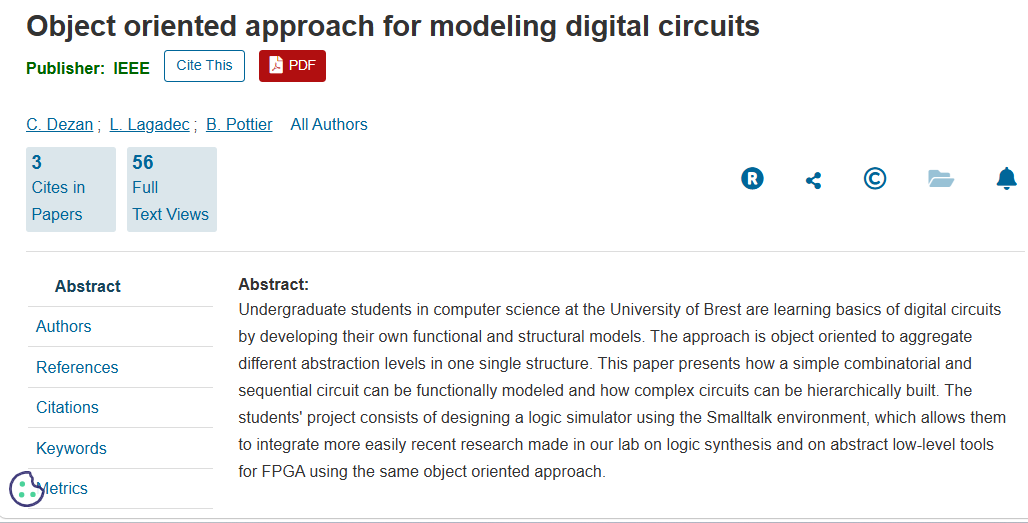
\includegraphics[width=0.9\textwidth, height=0.75\textheight, keepaspectratio]{image.png}
\end{center}

\newpage
\section{Proposed Work}
The primary objective of the proposed project is to develop a software simulator for digital circuits. The system will employ a strict object-oriented approach. This architecture will model both the functional and structural characteristics of electronic components. The core design relies on the methodologies proposed by Dezan, Lagadec, and Pottier. These authors demonstrate how to encapsulate multiple abstraction levels into a unified software structure. The proposed software will implement their functional object definitions for both combinatorial and sequential circuits. Furthermore, the system will execute their hierarchical method for building complex digital systems. The project will utilize the Java programming language. Java provides robust support for modern software design patterns. This technical choice ensures a highly modular and extensible codebase.

\subsection{Combinatorial Logic Modeling}
The simulator will translate foundational concepts from the reference literature into a practical Java implementation. First, the software will model combinatorial logic using discrete functional objects. A combinatorial circuit relies purely on its current input values to determine its output. The system will represent physical components like adders and basic logic gates as distinct software objects. These objects will contain specific methods to evaluate Boolean logic mathematically. The evaluation mechanism will read incoming binary signals. It will then apply the corresponding logical operations to generate an output. The software will process these functional blocks to derive accurate truth tables. A truth table represents all possible input combinations and their resulting outputs. This tabular representation allows the system to verify the functional correctness of the modeled circuit.

\subsection{Sequential Logic Modeling}
Second, the project will implement sequential circuits based on standard automata models. A sequential circuit uses both current inputs and internal memory states to determine outputs. The architecture will separate transition functions from output functions. The transition functions will update internal state variables synchronously. This synchronous update will occur upon receiving a master clock signal. The output functions will then evaluate asynchronously to generate the final electrical signal. This separation accurately mimics the physical behavior of components like flip-flops and counters. The software will maintain internal variables to track the current state of the automata. The simulation engine will evaluate these state blocks on explicit demand.

\subsection{Hierarchical Circuit Composition}
Third, the system will support hierarchical circuit composition. The reference paper describes building circuits by defining dependencies and nets. A net is a conductive wire connecting the inputs and outputs of different subcircuits. Each net carries a specific binary value during simulation. The software will continually monitor these nets for value changes. The reference implementation achieved this monitoring using explicit value holder constructs. The proposed Java system will replicate this behavior using the observer design pattern. This monitoring capability allows the simulator to cascade signal updates throughout the entire circuit hierarchy automatically. Consequently, a single input change will propagate naturally across all connected structural dependencies.

\subsection{Discrete Event Timing Engine}
The proposed project will expand upon the foundational models by introducing five novel architectural features. The first extension is a discrete event timing engine. Physical silicon gates require a small amount of time to process electrical signals. Engineers define this processing time as a propagation delay. The simulator will model this physical delay using a priority-based event queue. The software will schedule signal updates at specific future timestamps rather than evaluating them instantaneously. This temporal modeling provides a highly realistic representation of actual hardware behavior.

\subsection{Composite Module Encapsulation}
The second extension is a hierarchical composite module encapsulation system. The application will allow users to construct a complex circuit out of primitive logic gates. Users can then package this complex circuit into a single reusable software module. The software will treat this new composite module exactly like a basic logic gate. This approach builds directly upon the structural composition theories discussed in the reference literature. This feature ensures strict modularity and enables high code reuse across different simulated designs.

\subsection{Standardized Waveform Export}
The third extension involves an automated waveform export mechanism. The system will implement an observer design pattern to monitor signal transitions over simulated time. The software will record every voltage change and generate a Value Change Dump file. A Value Change Dump file is an industry standard text format for representing timing diagrams. Users can open this exported file in external visualization tools. This capability allows engineers to analyze circuit timing behavior visually.

\subsection{Hardware Fault Injection}
The fourth extension is a silicon defect fault injection engine. Manufacturing flaws often cause permanent short circuits in physical hardware. Engineers refer to these permanent errors as stuck at faults. The simulator will allow users to intentionally inject these faults into virtual wires. The system intercepts standard signal propagation and forces a permanent high or low voltage state. This diagnostic feature will help users verify if their input test patterns can successfully detect hidden hardware errors.

\subsection{Netlist Parsing}
The fifth extension is an external netlist parser. A netlist is a structured text document describing electronic components and their physical connections. The project will include a parser to read circuit structures from external configuration files. The software will dynamically instantiate the correct objects in memory based on this input data. This parser removes the need to hardcode circuit designs directly into the software source code.

\subsection{Execution Pipeline}
A strict execution pipeline will govern the entire simulation process. The pipeline begins with the initialization of the circuit structure. The parser reads the external configuration file. It then triggers object creation through dedicated factory classes. Next, the software validates the circuit topology. It scans the network graph to prevent illegal continuous feedback loops. After validation, the simulation clock begins tracking time. The engine processes queued signal events sequentially. Finally, the software outputs the resulting truth tables and timing waveforms. This structured approach guarantees predictable software execution and accurate simulation results.

\subsection{Final Deliverables}
The project will culminate in several distinct deliverables. The first deliverable is the complete Java source code for the simulation engine. The second deliverable comprises sample input netlist files and their corresponding output waveform files. These files will demonstrate the system functioning correctly under various test scenarios. The third deliverable is a comprehensive technical document. This document will specify the programming language version along with hardware requirements and software dependencies. It will also provide detailed instructions explaining how to view the software demonstration. The final deliverable is a comprehensive project report. This report will aggregate all system analysis models, design diagrams, and execution summaries into a single cohesive document.

\newpage

\section{System Analysis}

\subsection{System Concept and Problem Statement}
The proposed simulation framework addresses critical verification challenges in digital electronics design. Physical hardware prototyping introduces significant financial and temporal costs during the development lifecycle. Engineers require robust software utilities to verify logic topologies mathematically prior to manufacturing. The target demographic for this application includes academic researchers and digital systems engineers. The primary operational environment consists of a local desktop execution context. 

The architecture utilizes an event-driven engine to parse textual netlists. This engine subsequently initializes a priority event queue to cascade binary signals through virtual logic gates over simulated time. The formal problem statement dictates that the software must simulate signal propagation across a given netlist of logic gates and flip-flops. The system must also identify invalid combinational feedback loops. Finally, the application must generate accurate truth tables and precise timing waveforms.

\subsection{Requirements Modeling}
The system capabilities encompass both functional and non-functional requirements. Each functional requirement correlates directly with a defined use case and a structural methodology derived from the reference literature. 

\begin{table}[h!]
\centering
\renewcommand{\arraystretch}{1.3}
\begin{tabularx}{\textwidth}{|l|X|l|l|}
\hline
\textbf{ID} & \textbf{Functional Requirement} & \textbf{Priority} & \textbf{Use Case} \\ \hline
FR1 & The system shall parse external configuration files to construct an internal circuit object graph. & Must & UC-01 \\ \hline
FR2 & The validation module shall analyze the circuit topology to detect and prohibit unclocked combinational feedback loops. & Must & UC-02 \\ \hline
FR3 & The execution engine shall evaluate Boolean logic for primitive combinatorial gates using discrete mathematical models. & Must & UC-03 \\ \hline
FR4 & The engine shall update sequential states synchronously upon receiving a designated master clock signal. & Must & UC-04 \\ \hline
FR5 & The architecture shall support the encapsulation of primitive gates into reusable hierarchical composite modules. & Must & UC-05 \\ \hline
FR6 & The simulation shall model physical signal propagation delays via a discrete priority event queue. & Must & UC-06 \\ \hline
FR7 & The diagnostic module should allow the manual injection of permanent hardware faults onto designated interconnecting wires. & Should & UC-07 \\ \hline
FR8 & The application should export simulated signal transitions into a standardized waveform file format. & Should & UC-08 \\ \hline
\end{tabularx}
\end{table}

The architecture must evaluate composite modules and primitive gates uniformly to preserve the Open Closed Principle. The event processing queue must handle a minimum of ten thousand discrete signal events per second. The codebase must permit the integration of novel logic gate types through the addition of a single isolated class file. Furthermore, the domain logic and simulation engine must achieve eighty percent coverage via automated unit testing.

\subsection{Domain Analysis and Class Model}
The domain analysis phase translates physical hardware abstractions into discrete software entities. The noun extraction process identifies core components from the formal problem statement and the primary reference literature.
\begin{figure}[H]
    \centering
    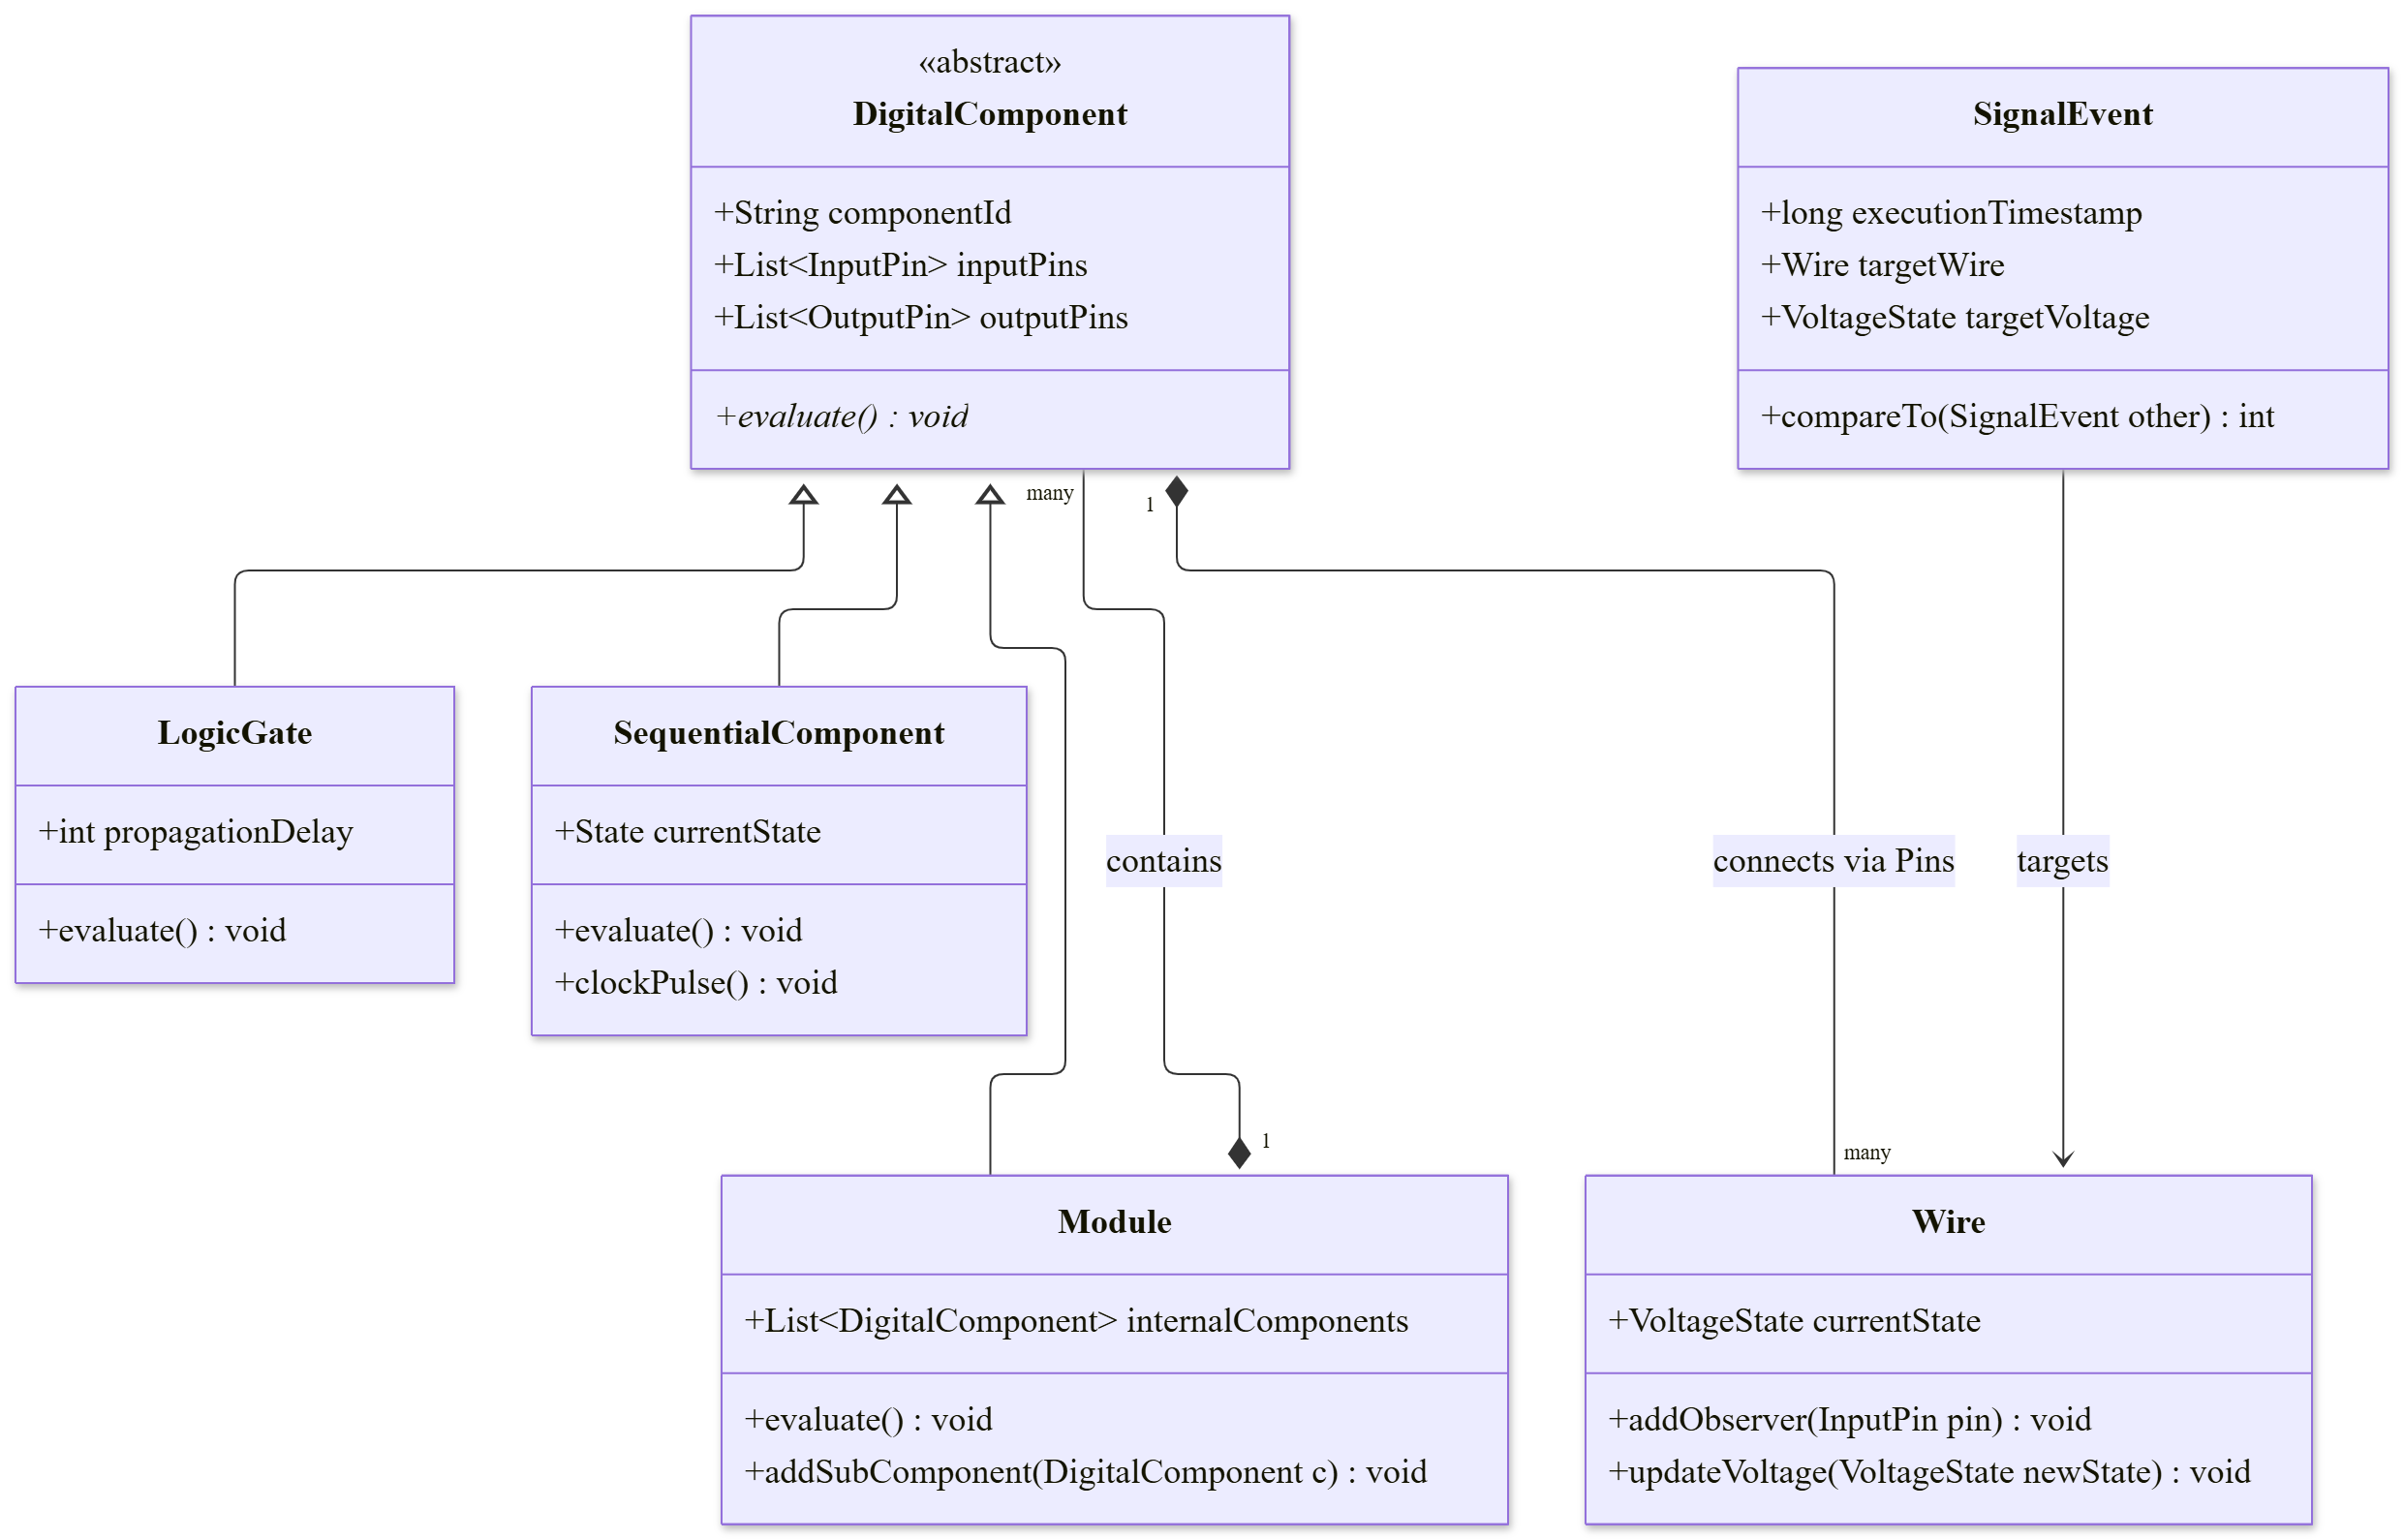
\includegraphics[width=\textwidth]{classDiagram.png}
    \caption{Class Diagram illustrating the architectural dependencies and structural relationships of the simulation domain entities.}
    \label{fig:class_diagram}
\end{figure}
\begin{table}[h!]
\centering
\renewcommand{\arraystretch}{1.3}
\begin{tabularx}{\textwidth}{|l|X|}
\hline
\textbf{Class Name} & \textbf{Scope and Responsibility in the System} \\ \hline
DigitalComponent & An abstract superclass representing any generalized circuit entity possessing input pins and an evaluation protocol. \\ \hline
LogicGate & A primitive structural unit that calculates outputs instantaneously based on foundational Boolean algebra. \\ \hline
SequentialComponent & A stateful hardware model containing internal memory allocations that update strictly synchronously. \\ \hline
Module & A composite architectural container encapsulating multiple nested components to function as a singular integrated unit. \\ \hline
Wire & A conductive topological link connecting an output source to one or multiple input destinations. \\ \hline
SignalEvent & A discrete temporal object encapsulating a binary state transition targeted for a specific execution timestamp. \\ \hline
\end{tabularx}
\end{table}


The structural relationships among these domain entities rely heavily on classical inheritance and composition hierarchies. The corresponding class diagram visually articulates these architectural dependencies.


\subsection{Domain Analysis and State Model}
The state model defines the distinct operational phases of the primary simulation controller. Combinatorial logic gates do not retain independent operational states. Conversely, the core execution engine transitions through a strict lifecycle to ensure deterministic behavior. The simulation engine initializes in an idle configuration. The system transitions into a parsing state upon receiving an external netlist configuration file. The software subsequently enters a validation state to ensure topological integrity. The engine then transitions into the active execution loop. The simulation process formally terminates upon depleting the priority event queue.

\begin{figure}[H]
\centering
% \begin{mermaid}
% stateDiagram-v2
%     [*] --> Idle
%     Idle --> Parsing : loadNetlist()
%     Parsing --> Validating : netlistParsed
%     Validating --> Executing : validationPassed
%     Validating --> Failed : cycleDetected
%     Executing --> Terminated : queueEmpty
%     Executing --> Terminated : maxTimeReached
%     Failed --> [*]
%     Terminated --> [*]
% \end{mermaid}
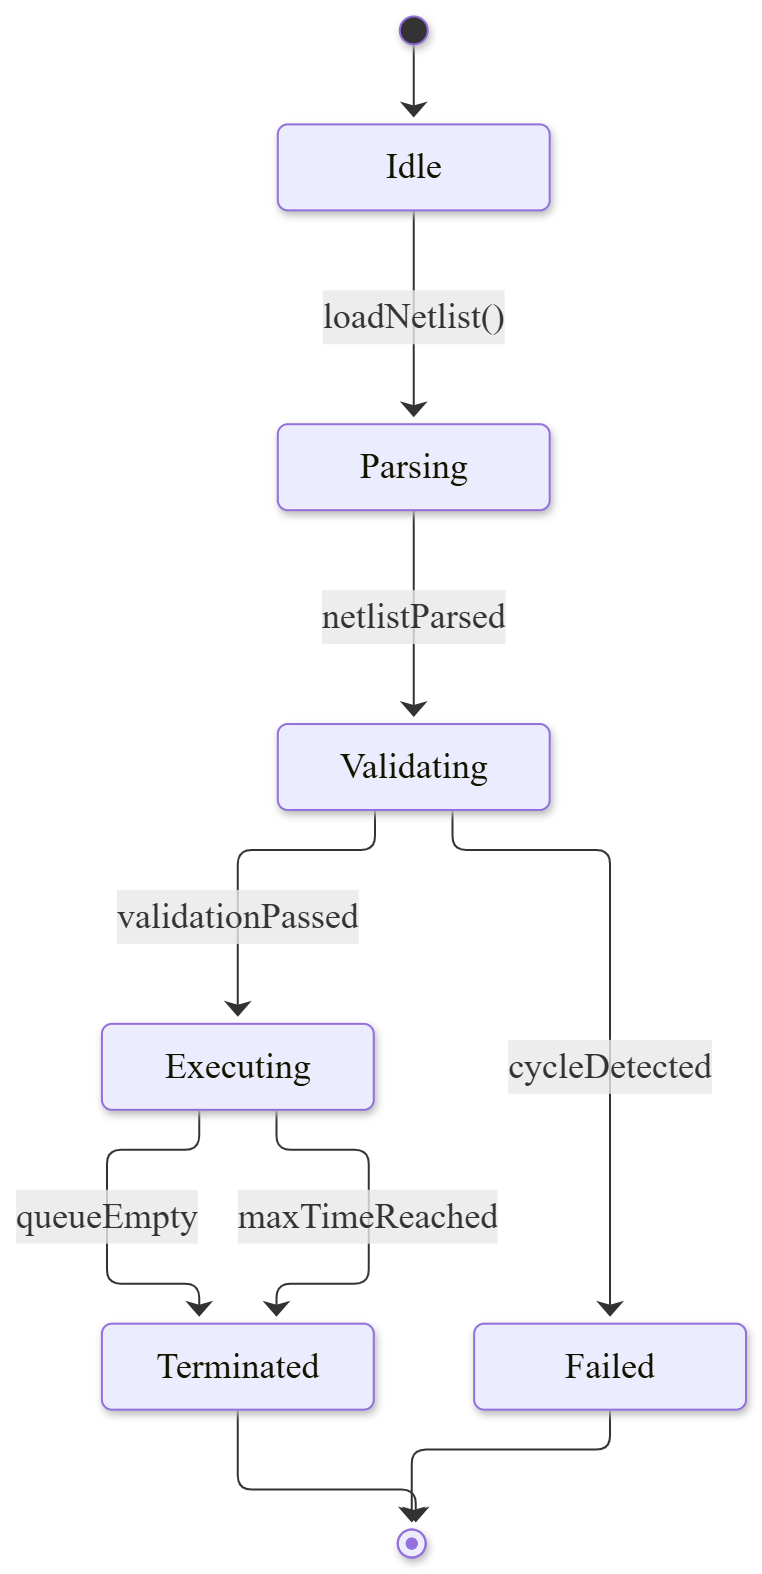
\includegraphics[width=\textwidth, height=0.4\textheight, keepaspectratio]{stateDiagram.png}

\caption{State Diagram representing the lifecycle of the Simulation Engine.}
\end{figure}

\subsection{Application Analysis and Interaction Model}
The interaction model defines the boundary between the external human actor and the internal software logic. The primary actor is the electronics engineer. The engineer interacts with the system through an abstract command interface. The application isolates the internal domain logic from the external data sources. The most critical interaction sequence involves executing a full simulation batch. 

\begin{table}[h!]
\centering
\renewcommand{\arraystretch}{1.3}
\begin{tabularx}{\textwidth}{|>{\raggedright\arraybackslash}p{3cm}|X|}
\hline
\textbf{Attribute} & \textbf{Specification for UC-06: Execute Simulation} \\ \hline
Initial Event & The user issues a command to execute a simulation for a specific netlist. \\ \hline
Main Scenario & 1. The system loads the netlist and instantiates components. \newline 2. The system validates the topology. \newline 3. The simulation clock initializes at zero. \newline 4. The engine processes queued signal events sequentially. \newline 5. The system aggregates the final states. \newline 6. The software returns the generated waveform file. \\ \hline
Exceptions & 1a. The netlist format is invalid. The system aborts and reports an error. \newline 2a. The system detects an unclocked combinational loop. The engine rejects the topology. \\ \hline
Business Rules & The system must evaluate unclocked combinational gates instantaneously. The system must evaluate sequential gates synchronously based on the master clock. \\ \hline
\end{tabularx}
\end{table}

The interaction sequence requires a strict chronological flow of messages between software boundaries. The following sequence diagram illustrates the internal method calls during a standard simulation run.

\begin{figure}[h!]
\centering
% \begin{mermaid}
% sequenceDiagram
%     actor User
%     participant Facade as SimulationFacade
%     participant Engine as EventEngine
%     participant Validator as TopologyValidator
%     participant Gate as LogicGate
    
%     User->>Facade: executeSimulation(netlist)
%     Facade->>Engine: initialize(netlist)
%     Engine->>Validator: checkCycles()
%     Validator-->>Engine: validationPassed
    
%     loop Until Queue Empty
%         Engine->>Engine: dequeueNextEvent()
%         Engine->>Gate: evaluate()
%         Gate-->>Engine: scheduleNewEvent(time + delay)
%     end
    
%     Engine-->>Facade: simulationComplete
%     Facade-->>User: return WaveformFile
% \end{mermaid}
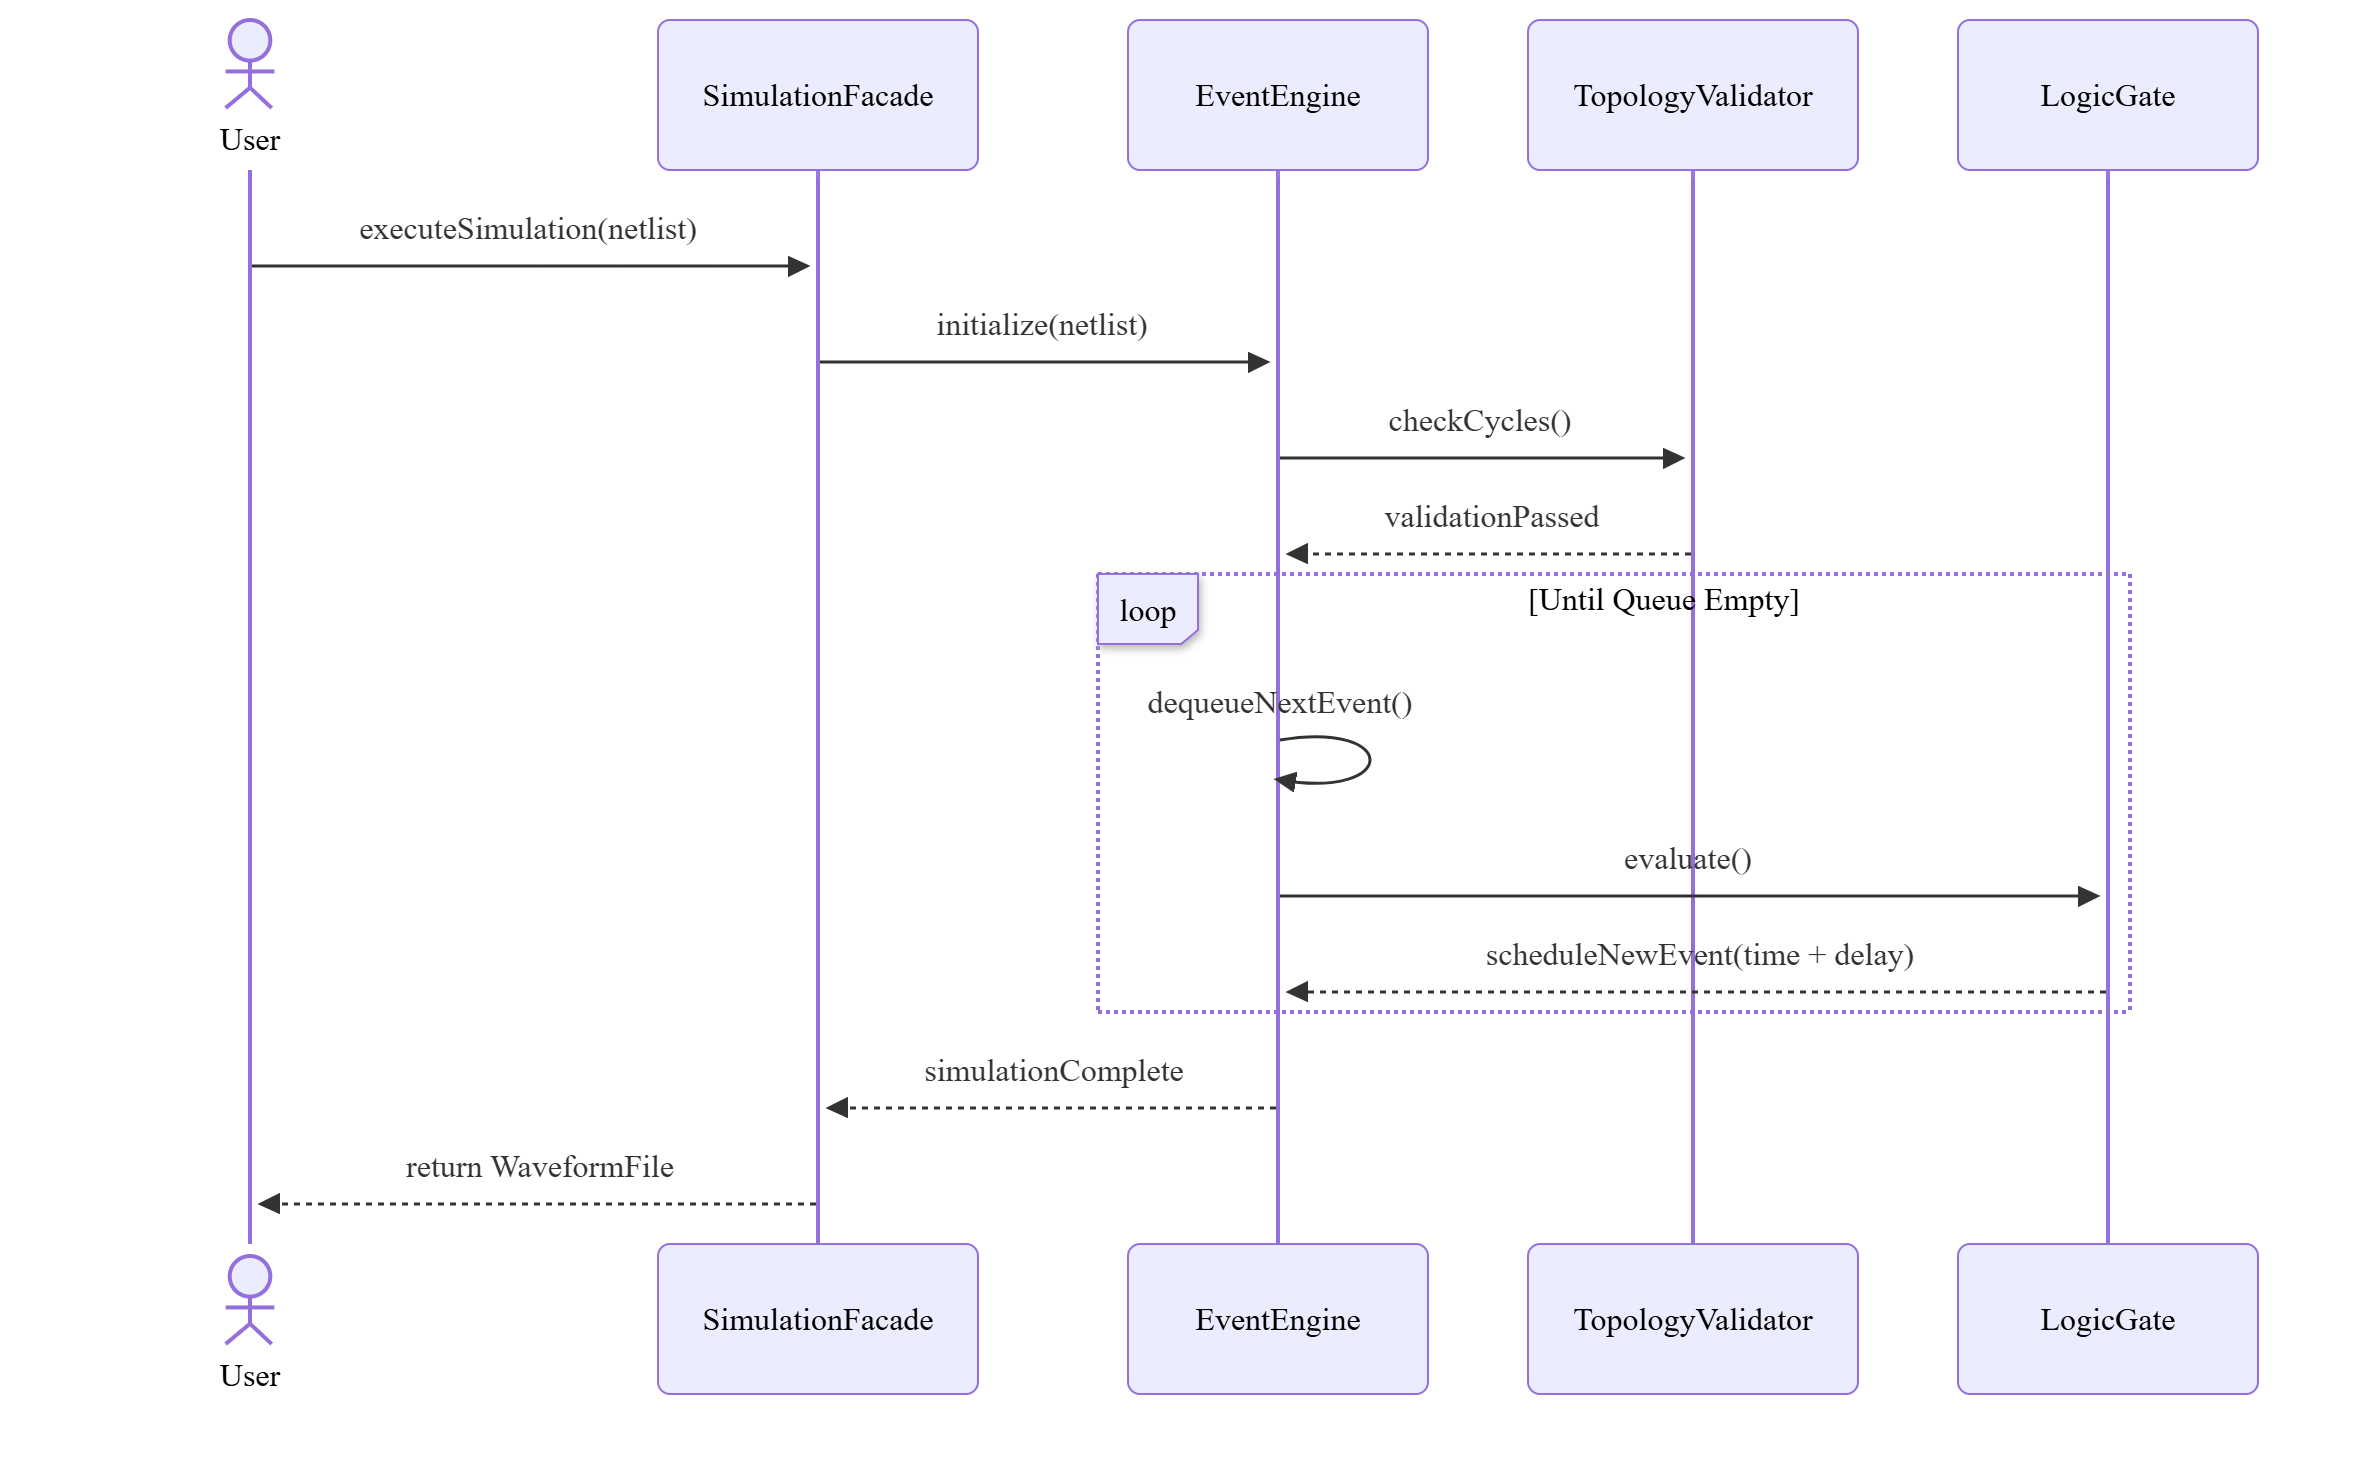
\includegraphics[width=\textwidth]{sequenceDiagram.png}
\caption{Sequence Diagram illustrating the method calls during simulation execution.}
\end{figure}

The physical evaluation of a digital component requires specific logical branching. The activity diagram visualizes this concurrent evaluation process.

\begin{figure}[H]
\centering
% \begin{mermaid}
% flowchart TD
%     A[Start Evaluation] --> B{Is Component Sequential?}
%     B -- Yes --> C[Wait for Clock Edge]
%     C --> D[Update Internal State]
%     D --> E[Output New Signal]
    
%     B -- No --> F[Read Input Pins]
%     F --> G[Apply Boolean Logic]
%     G --> H{Did Output Change?}
    
%     H -- Yes --> I[Schedule Event with Delay]
%     H -- No --> J[Drop Event]
    
%     E --> K[End Evaluation]
%     I --> K
%     J --> K
% \end{mermaid}
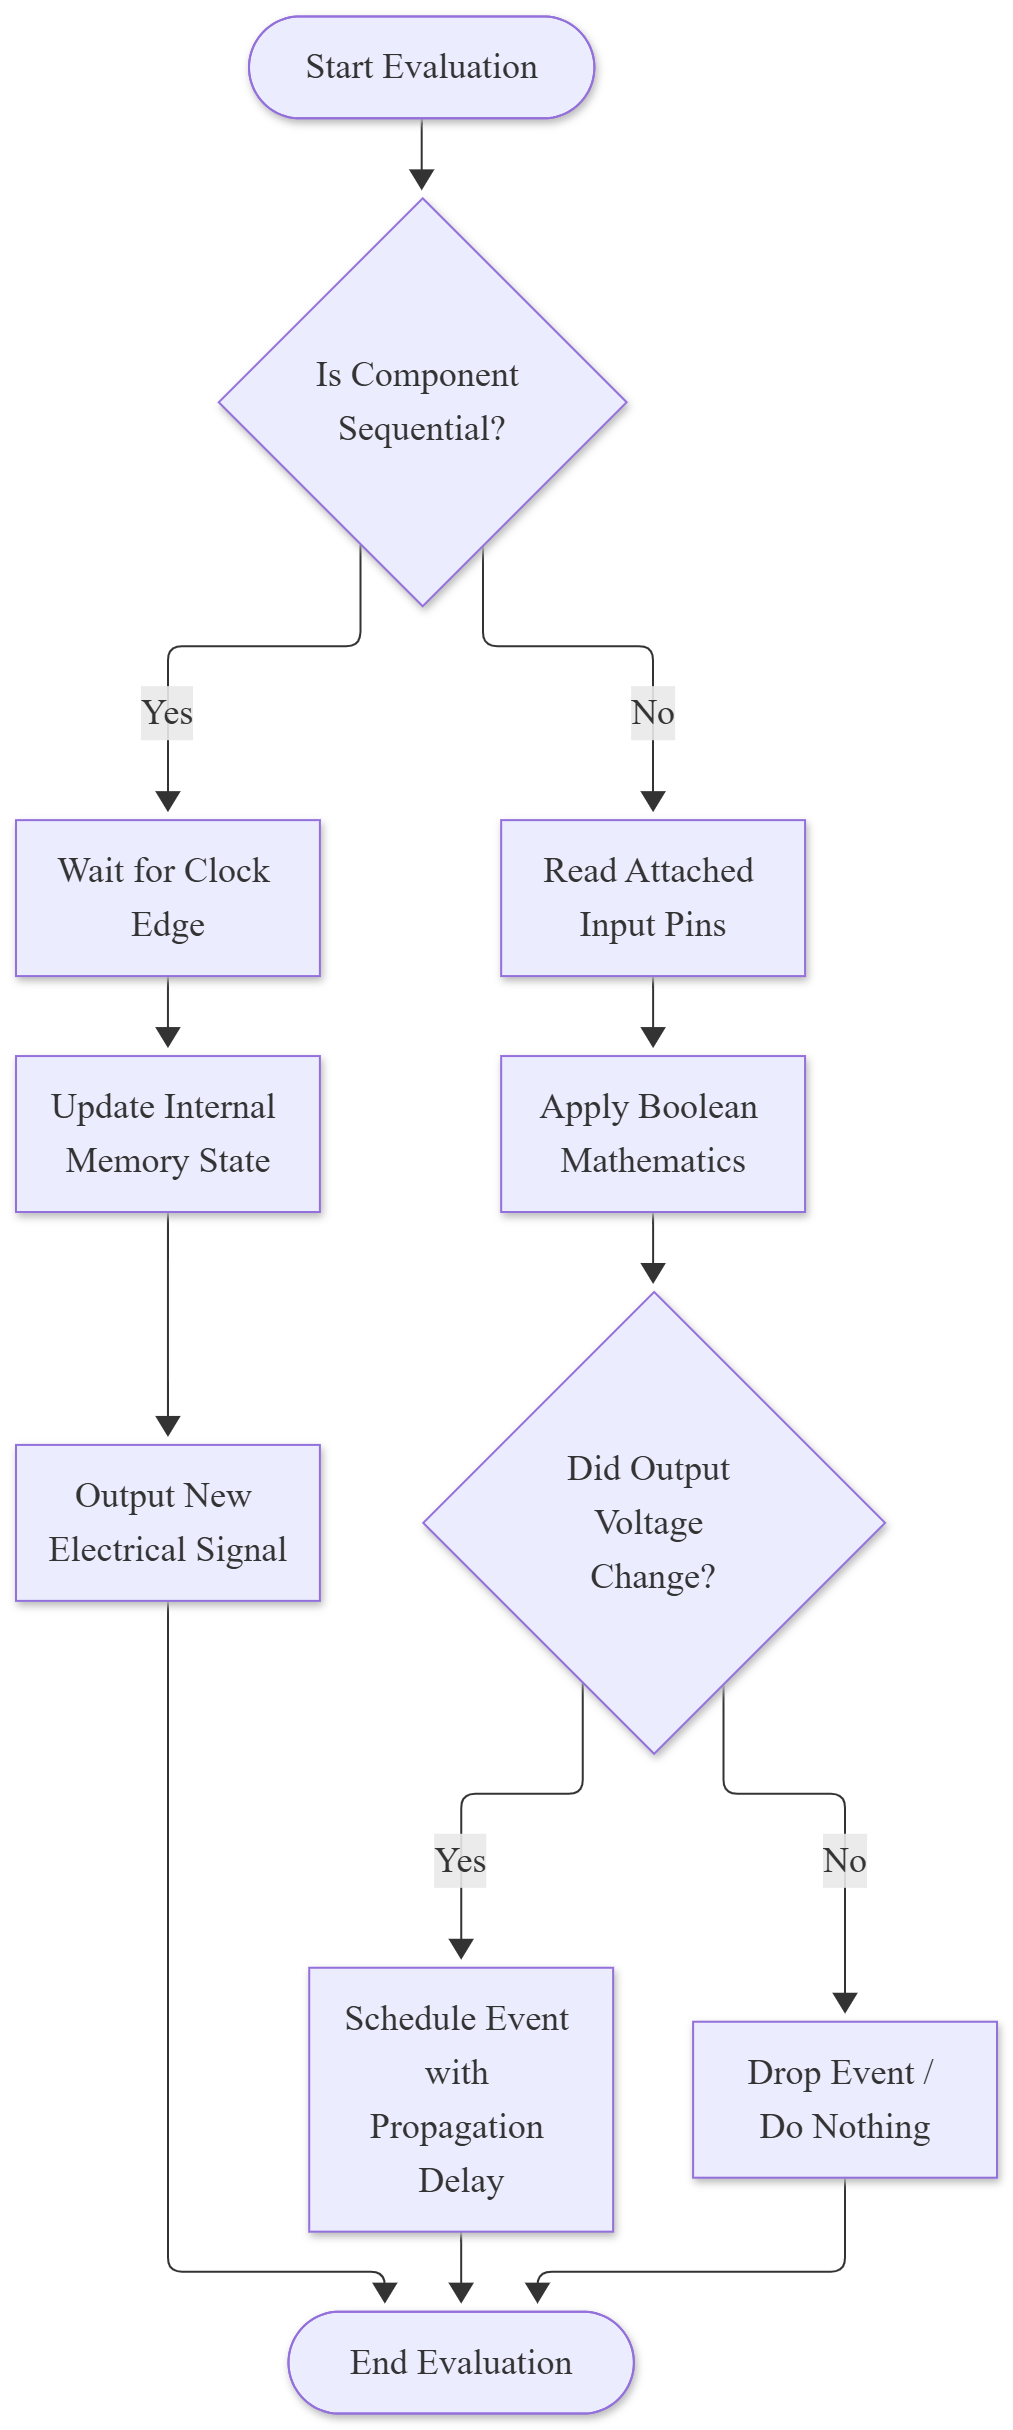
\includegraphics[width=\textwidth, height=0.4\textheight, keepaspectratio]{activityDiagram.png}
\caption{Activity Diagram detailing the evaluation logic for a Digital Component.}
\end{figure}

\subsection{Consistency Checks and Assumptions}
The consistency analysis verifies the architectural cohesion of the proposed object-oriented design. The design successfully maps every functional requirement to a dedicated software class. The proposed \textit{DigitalComponent} interface successfully fulfills the requirement for uniform evaluation methodologies. The event parameters map directly to the attributes defined within the \textit{SignalEvent} class structure.

The system architecture relies upon specific technical assumptions. The engine assumes a strictly single-threaded execution environment for the priority event queue. This single-threaded assumption prevents race conditions during state evaluations. This architecture guarantees deterministic simulation results across multiple executions. The project constraints assume the developer will implement standard testing scenarios utilizing synthetic datasets.


\section{Potential Use of Patterns}
The software architecture heavily leverages standard object-oriented design patterns. These patterns ensure structural modularity across the codebase. They also enforce high cohesion and reduce coupling between independent software components. The development process applies five specific Gang of Four design patterns to resolve distinct architectural challenges.

\subsection{Observer Pattern for Signal Propagation}
The first architectural challenge involves signal propagation. Signal updates must propagate automatically through the interconnected circuit. Logic gates cannot constantly poll each other for voltage changes. Constant polling would severely degrade simulation performance. The system solves this computational inefficiency using the Observer pattern. A conductive wire acts as the primary observable subject. The connected input pins act as registered observers. A wire changes its internal electrical state. The wire then instantly notifies all attached input pins. This notification triggers downstream logic gate evaluations automatically. This event-driven approach ensures optimal performance and eliminates redundant processing cycles.

\subsection{Composite Pattern for Structural Uniformity}
The second architectural challenge involves structural complexity. The system must process individual logic gates and complex multi-gate circuits uniformly. Evaluating a single logic gate should require the exact same method call as evaluating a massive processing module. The system achieves this necessary uniformity by utilizing the Composite pattern. Both primitive logic gate objects and complex module objects implement an identical component interface. The simulation engine simply calls the evaluation method on any given component. The engine never needs to know the internal structural complexity of the target object. This abstraction allows developers to build infinitely nested circuit hierarchies.

\subsection{Factory Method Pattern for Dynamic Instantiation}
The third architectural challenge involves component instantiation. Hardcoding object creation restricts software extensibility. Adding new logic gate types would require modifying the core engine code. The system resolves this structural limitation using the Factory Method pattern. A dedicated component factory dynamically instantiates logic gate objects during the initial netlist parsing phase. The factory reads specific string identifiers from the configuration file. It then creates the appropriate software objects in memory. This dynamic creation approach perfectly satisfies the Open Closed Principle. Developers can introduce new gate components without altering the existing factory logic.

\subsection{Singleton Pattern for Temporal Synchronization}
The fourth architectural challenge involves temporal synchronization. Sequential circuits require a single universally synchronized timeline. Multiple simulation clocks running independently would corrupt the global state. The system prevents this data corruption using the Singleton pattern. The software implements the simulation clock and the central event scheduler as strict Singletons. This design guarantees that exactly one centralized timeline dictates all synchronous state transitions globally. Every sequential component references this single clock instance to coordinate memory updates.

\subsection{State Pattern for Memory Encapsulation}
The fifth architectural challenge involves memory encapsulation. Sequential hardware components like flip-flops possess internal memory. This internal memory drastically alters their behavioral output over simulated time. The system models this dynamic hardware behavior utilizing the State pattern. A sequential component delegates its evaluation logic to dedicated internal state objects. The component behaves differently depending on its current internal state configuration. This structural delegation cleanly separates the state transition functions from the physical output generation. The system can easily transition between high and low memory states by swapping the active state object.

\section{How to Approach a Solution}
The development process requires a highly structured methodology to ensure successful implementation. The execution pipeline is divided into five sequential computational phases. These discrete phases isolate specific software responsibilities. This isolation ensures predictable software execution and generates accurate analytical results.

\subsection{Development Methodology and Testing Strategy}
The developer will implement the system utilizing an iterative software development methodology. The project relies strictly on a use case driven approach characteristic of the Unified Process. The developer will build the most valuable and high risk features during the earliest iterations. This iterative strategy ensures a functional core system exists well before the final deadline. The project will also incorporate test driven development principles. The developer will write automated unit tests prior to implementing the core domain rules. These automated tests will verify the functional correctness of individual logic gates and the priority event queue.

\subsection{Phase One: Netlist Parsing and Instantiation}
The application initiates the pipeline by loading an external configuration file. This file contains the complete topographical definition of the digital circuit. The parsing module reads this document sequentially. It utilizes the Factory Method pattern to instantiate the corresponding Java objects. The system creates distinct objects for logic gates, connection pins, and conductive wires. The software then links these objects in memory to construct the final directed circuit graph.

\subsection{Phase Two: Topology Validation}
The validation algorithm must traverse the generated object graph before the simulation begins. The algorithm performs a rigorous cycle detection scan. This scan ensures the circuit contains no illegal combinational feedback loops. An unclocked loop would cause an infinite evaluation cycle and crash the software. The system also verifies standard physical constraints. It ensures that multiple output pins do not attempt to drive the exact same wire simultaneously.

\subsection{Phase Three: Engine Initialization}
The simulation engine initializes the master clock and the priority event queue. The software requires initial boundary conditions to begin the simulation. The user provides these initial test stimulus values within the configuration file. The system injects these initial voltage values into the event queue at timestamp zero. The computational environment is then fully prepared to process sequential events.

\subsection{Phase Four: Discrete Event Loop}
The core engine executes the discrete event loop continuously. The engine dequeues the earliest scheduled signal event from the priority queue. It updates the target wire immediately. Downstream logic gates receive this update via the Observer pattern. The affected gates evaluate their internal Boolean logic. A gate schedules a new signal event in the queue if its calculated output changes. The engine offsets the timestamp of this new event by the specific physical propagation delay of the particular gate.

\subsection{Phase Five: Output Generation}
The execution loop concludes once the event queue becomes empty. The loop will also terminate if the simulation reaches a predefined maximum time limit. The system generates final analytical reports upon termination. It prints a complete logic truth table to the standard console. The software simultaneously flushes the waveform logger data to the physical hard disk. This action generates a standardized timing file. The user can subsequently open this file in specialized graphical viewing software to analyze the timing behavior visually.
\section{References}

C. Dezan, L. Lagadec, B. Pottier; Object oriented approach for modeling digital circuits; Proceedings 1999 IEEE International Conference on Microelectronic Systems Education (MSE'99); Arlington, VA, USA; 1999, pp. 51-52.

\end{document}